% Provenance (never printed): see sources/outline_sources.md (Year 3:
% moments of inertia and gravity fields; impact cratering and crater dating;
% volcanism and tectonics on Mars, Venus, Io and the icy moons).
% Brief: sources/book5/BRIEFS.md, ch. 26. Curves from figdata/bachelor-3/
% two_layer_planet.py (two-layer interiors of the Earth, Mars, the Moon and
% Mercury from mean density and moment of inertia) and crater_sfd.py
% (the Ivanov production function and the Hartmann-Neukum chronology of
% Mars from the Craterstats configuration, the lunar chronology of Neukum,
% Hartmann's equilibrium density, and two invented Martian plains whose
% counts are drawn once from a Poisson law). Exercise and problem values in
% the Book 5 scratch calculator calc/ch26.py. Plains A and B are invented.
\chapter{ग्रहीय अंतरंग और सतहें}\label{ch:b3:planetary-interiors-surfaces}

दूरबीन से देखने पर चंद्रमा की दो प्रकार की सतहें दिखती हैं। चमकीली
उच्चभूमियाँ क्रेटरों से ढकी हैं, क्रेटर पर क्रेटर: वे एक तीव्र बमबारी द्वारा
बड़े क्रेटरों से संतृप्त कर दी गई थीं, वह बमबारी जो लगभग 3.8 अरब
वर्ष पहले समाप्त हुई। गहरे रंग के मारिया, जो 4.2 और 1.2 अरब
वर्ष पहले के बीच लावा से भरे मैदान हैं, उनमें क्रेटर कहीं कम हैं। अपोलो और लूना
मिशनों ने दोनों से चट्टानें लौटाईं, और उनकी रेडियोमेट्रिक आयुओं ने
किसी सतह पर क्रेटरों के घनत्व को एक घड़ी में बदल दिया। यह घड़ी अब मंगल, बुध
और बर्फीले उपग्रहों के मैदानों की तिथि निर्धारित करती है, जिनसे अभी तक कोई चट्टान
वापस नहीं लाई गई है। यह अध्याय ग्रहों के अंतरंगों को उनके गुरुत्व,
घूर्णन और ज्वारों में पढ़ता है, फिर उनकी सतहों को उनके क्रेटरों,
ज्वालामुखियों और भ्रंशों में।
% ledger: french:highlands, nasa:moon-core, marchi:neukum

\begin{recall}
जड़त्व-आघूर्ण गुणक $C = I/MR^2$, इससे और माध्य घनत्व से बना ग्रह का दो-परत मॉडल,
स्थलीय और विशाल ग्रह पुस्तक 3 (स्नातक वर्ष 1) में हैं, उसके तुलनात्मक
ग्रहविज्ञान वाले अध्याय में; प्रावार-स्तंभ और बृहत आग्नेय प्रांत
उसके हॉटस्पॉट वाले अध्याय में हैं। ग्रहीय विभेदन और उल्कापिंड
पुस्तक 4 (स्नातक वर्ष 2) में हैं, ग्रह-निर्माण वाले अध्याय में।
\omterm{def:b3:gravity-geodesy:j2}{गतिक रूप-गुणक} $J_2$, \omterm{thm:b3:gravity-geodesy:maccullagh}{मैककला सूत्र} और \omterm{def:b3:gravity-geodesy:flexure}{स्थलमंडलीय आनमन} इस पुस्तक में
उसके गुरुत्व और भूगणित वाले अध्याय में हैं; \omterm{def:b3:mantle-convection:rayleigh}{रैले संख्या}
प्रावार संवहन वाले अध्याय में है। ज्वार, केप्लर के नियम और
प्रत्यास्थ मापांक भौतिकी की पुस्तकों में हैं;
पॉइसन बंटन
गणित की पुस्तकों में है।
\end{recall}

\section{गुरुत्व, घूर्णन और ज्वारों से अंतरंग}\label{sec:b3:planetary-interiors-surfaces:interiors}

किसी ग्रह का द्रव्यमान, जो किसी उपग्रह या अंतरिक्ष यान की कक्षा से प्राप्त होता है, उसका माध्य घनत्व देता है;
उसके अक्ष का पुरस्सरण और उसका $J_2$ उसके जड़त्व
आघूर्ण देते हैं। पुस्तक 3 (स्नातक वर्ष 1) का दो-परत प्रस्ताव इन दोनों
संख्याओं को एक क्रोड में बदल देता है, परंतु केवल तब जब प्रावार का घनत्व चुन लिया जाए:
दो मापन तीन अज्ञात राशियों को निश्चित नहीं कर सकते।

\begin{omfigure}
\centering
\begin{tikzpicture}
\begin{axis}[width=0.78\linewidth, height=0.46\linewidth,
  xmin=3000, xmax=16000, ymin=0, ymax=1,
  xlabel={क्रोड घनत्व $\rho_c$ (\unit{kg.m^{-3}})},
  ylabel={क्रोड त्रिज्या / ग्रह त्रिज्या $x$},
  tick label style={font=\scriptsize}, label style={font=\small},
  scaled x ticks=false, xtick={4000,6000,8000,10000,12000,14000,16000},
  xticklabels={4000,6000,8000,10\,000,12\,000,14\,000,16\,000}]
\addplot[thick, omDef] table[x=rho_c, y=x] {figdata/out/bachelor-3-two_layer_planet-curve-Earth.dat};
\addplot[thick, red!70!black] table[x=rho_c, y=x] {figdata/out/bachelor-3-two_layer_planet-curve-Mars.dat};
\addplot[thick, black!60, dashed] table[x=rho_c, y=x] {figdata/out/bachelor-3-two_layer_planet-curve-Moon.dat};
\addplot[thick, orange!80!black] table[x=rho_c, y=x] {figdata/out/bachelor-3-two_layer_planet-curve-Mercury.dat};
\addplot[only marks, mark=*, mark size=2pt, black] table[x=rho_c, y=x] {figdata/out/bachelor-3-two_layer_planet-points.dat};
\node[font=\scriptsize, omDef, anchor=south west] at (axis cs:12600,0.55) {पृथ्वी};
\node[font=\scriptsize, red!70!black, anchor=south west] at (axis cs:6600,0.55) {मंगल};
\node[font=\scriptsize, black!70, anchor=south west] at (axis cs:11000,0.2) {चंद्रमा};
\node[font=\scriptsize, orange!80!black, anchor=south west] at (axis cs:7300,0.83) {बुध};
\end{axis}
\end{tikzpicture}
\par\smallskip{\small माध्य घनत्व और चार पिंडों के जड़त्व-आघूर्ण गुणक से अनुमत दो-परत मॉडल:
प्रत्येक वक्र संभावित प्रावार घनत्वों पर चलता है; अधिक घनत्व वाला प्रावार छोटा और सघन
क्रोड छोड़ता है। बिंदु मापी गई क्रोड त्रिज्याएँ दर्शाते हैं: पृथ्वी की भूकंपविज्ञान से,
मंगल की इनसाइट भूकंपमापी से, चंद्रमा का आंतरिक क्रोड और द्रव
खोल, और बुध का मापन MESSENGER
अंतरिक्ष यान के गुरुत्व क्षेत्र से
किया गया।}\label{fig:b3:planetary-interiors-surfaces:two-layer}
\end{omfigure}
% ledger: planet:Earth.density, planet:Mars.density, planet:Moon.density, planet:Mercury.density, earth:MoI, nasa:mars, nasa:moon, nasa:mercury, data:prem, jpl:insight-interior, nasa:moon-core, agu:mercury-core

हर ग्रह एक वक्र देता है, बिंदु नहीं। मंगल के लिए क्रोड त्रिज्या
\qty{1830}{km} इनसाइट द्वारा मापी गई, \qty{3460}{kg.m^{-3}} का प्रावार
और \qty{6460}{kg.m^{-3}} का क्रोड चुनती है। बुध के लिए लगभग
\qty{2000}{km} त्रिज्या वाला क्रोड त्रिज्या का 82~प्रतिशत भरता है। चंद्रमा का वक्र
लगभग समतल है: उसका $C = 0.394$ इतना $\tfrac25$ के निकट है कि एक छोटा क्रोड
किसी भी घनत्व का हो, फिट बैठता है, और $0.001$ के बराबर $C$ का परिवर्तन क्रोड त्रिज्या को
दो गुने से अधिक खिसका देता है (\cref{exo:b3:planetary-interiors-surfaces:10} देखिए)।
अकेला गुरुत्व छोटे क्रोड को नहीं देख सकता; ज्वार और भूकंपीय तरंगें देख सकती हैं।
% ledger: jpl:insight-interior, agu:mercury-core, nasa:moon

\begin{definition}[लव संख्या]\label{def:b3:planetary-interiors-surfaces:love-number}
जब किसी ग्रह पर घात~2 का ज्वारीय विभव कार्य करता है, तो ग्रह विकृत होता है और
उसका पुनर्वितरित द्रव्यमान अपना एक विभव जोड़ता है। \emph{लव
संख्या}\index{लव संख्या} $k_2$ उस जुड़े विभव का ज्वारीय विभव से अनुपात है,
दोनों ग्रह की सतह पर मापे गए।
\end{definition}

एक दृढ़ ग्रह में $k_2 = 0$ होता है; समान घनत्व वाला द्रव ग्रह
पूरी तरह झुकता है, $k_2 = \tfrac32$ के साथ। इन दोनों के बीच यह संख्या मापती है कि
ग्रह का कितना भाग झुक जाता है।

\begin{proposition}[समान प्रत्यास्थ गोले की लव संख्या]\label{prop:b3:planetary-interiors-surfaces:kelvin}
समान घनत्व $\rho$, त्रिज्या $R$ और पृष्ठ-गुरुत्व $g$ वाला एक असंपीड्य गोला,
जिसकी दृढ़ता $\mu$ है, उसके लिए निम्न प्राप्त होता है:
\[
  k_2 = \frac{3/2}{1 + \dfrac{19\mu}{2\rho g R}} .
\]
\end{proposition}

यह परिणाम केल्विन का है और इसे स्वीकार किया जाता है। अनुपात $\mu/\rho gR$ प्रत्यास्थ दृढ़ता की
उस स्व-गुरुत्व से, जो ज्वारीय उभार को वापस खींचता है,
तुलना करता है: छोटे ग्रह कठोर होते हैं, बड़े ग्रह झुक जाते हैं। मंगल के लिए, $\rho gR =
\qty{4.97e10}{Pa}$; पृथ्वी के ऊपरी प्रावार की दृढ़ता के साथ,
संदर्भ पृथ्वी मॉडल में \qty{80}{km} गहराई पर \qty{67}{GPa} की, सूत्र
$k_2 = 0.109$ देता है। मंगल ग्लोबल सर्वेयर ऑर्बिटर के अनुरेखण ने
मंगल का सौर ज्वार मापा: $k_2 = 0.153 \pm 0.017$, जो
एक ठोस लौह क्रोड के लिए बहुत बड़ा है। कम से कम क्रोड का बाहरी भाग
द्रव है, और उसकी त्रिज्या 2003 में 1520 और \qty{1840}{km} के बीच रखी गई थी।
% ledger: nasa:mars, const:G, data:prem, yoder:mars-k2

भूकंपमापियों ने प्रश्न का निपटारा कर दिया। इनसाइट लैंडर ने
मंगलकंप रिकॉर्ड किए और क्रोड के शीर्ष से परावर्तित तरंगों का पता लगाया: त्रिज्या
\qty{1830}{km}, जो \qty{1560}{km} गहरे प्रावार और 20 से
\qty{37}{km} मोटी भूपर्पटी के नीचे है। चंद्रमा पर अपोलो अंतरिक्षयात्रियों द्वारा
लगाए गए भूकंपमापियों ने चंद्रकंप रिकॉर्ड किए, जिनमें सबसे गहरे, सैकड़ों
किलोमीटर नीचे के, पृथ्वी के ज्वारों से उत्पन्न हुए थे। चंद्रमा के क्रोड का अब
इस प्रकार वर्णन किया जाता है: \qty{240}{km} त्रिज्या का ठोस, लौह-समृद्ध आंतरिक क्रोड,
उसके चारों ओर \qty{90}{km} मोटा द्रव लौह कवच,
और उसके ऊपर आंशिक रूप से गलित एक परत।
% ledger: jpl:insight-interior, nasa:moonquakes, nasa:moon-core

\section{संघट्ट क्रेटरण}\label{sec:b3:planetary-interiors-surfaces:impacts}

अंतरिक्ष से आया कोई पिंड ग्रह से कम से कम उसके पलायन वेग पर टकराता है
(पृथ्वी के लिए \qty{11.2}{km.s^{-1}}); क्षुद्रग्रह प्रायः पृथ्वी से
15 से \qty{25}{km.s^{-1}} के वेग से, और धूमकेतु अधिकतम
\qty{60}{km.s^{-1}} तक के वेग से टकराते हैं। \qty{20}{km.s^{-1}} पर प्रत्येक किलोग्राम
\qty{2e8}{J} ऊर्जा वहन करता है, जो विस्फोटक के एक किलोग्राम की ऊर्जा से लगभग पचास गुना है।
यह संघट्ट भूमि में और प्रक्षेप्य में एक आघात-तरंग भेजता है;
प्रक्षेप्य पिघलकर वाष्पित हो जाता है, और आघात के पीछे चट्टान बाहर की ओर
गति में डाल दी जाती है, और कुछ सेकंडों में एक क्रेटर खुल जाता है।
% ledger: french:velocities, french:table21

\begin{definition}[क्षणिक क्रेटर, सरल क्रेटर, जटिल क्रेटर, इजेक्टा-आवरण]\label{def:b3:planetary-interiors-surfaces:crater-morphology}
\emph{क्षणिक क्रेटर}\index{क्षणिक क्रेटर} वह कटोरे-आकार की गुहा है
जो उत्खनन-प्रवाह द्वारा उस क्षण खुलती है जब उसका बढ़ना रुकता है; उसकी गहराई
उसके व्यास की लगभग एक-तिहाई होती है। एक \emph{सरल
क्रेटर}\index{सरल क्रेटर} उभरे किनारे वाला एक कटोरा है, जिसमें क्षणिक
क्रेटर मुश्किल से बदला है, और उसकी खड़ी दीवारें अंदर की ओर ब्रेशिया के एक लेंस में ढह जाती हैं।
एक \emph{जटिल क्रेटर}\index{जटिल क्रेटर} एक बड़ा क्रेटर है
जिसका क्षणिक कटोरा ध्वस्त हो गया: तल एक केंद्रीय उत्थान में ऊपर उठ गया, किनारा
वेदिकाओं के साथ अंदर की ओर खिसक गया, और तल समतल है। \emph{इजेक्टा-
आवरण}\index{इजेक्टा-आवरण} वह उत्खनित चट्टान की परत है, जो किनारे से परे
फेंकी गई और क्रेटर के चारों ओर जमा हुई।
\end{definition}
% ledger: french:transient, french:transition

\begin{omfigure}
\centering
\begin{tikzpicture}[x=0.55cm, y=0.55cm, font=\scriptsize, >=stealth]
\def\simpleprofile{(-6,0) -- (-3.6,0) .. controls (-3.0,0.45) .. (-2.6,0.55) .. controls (-1.8,-2.6) and (1.8,-2.6) .. (2.6,0.55) .. controls (3.0,0.45) .. (3.6,0) -- (6,0)}
\def\complexprofile{(-7,0) -- (-5.4,0) -- (-4.6,0.5) -- (-4.0,-0.3) -- (-3.6,-0.25) -- (-3.1,-1.0) -- (-2.7,-0.95) -- (-2.3,-1.5) -- (-0.8,-1.5) -- (-0.5,-0.6) -- (0,-0.3) -- (0.5,-0.6) -- (0.8,-1.5) -- (2.3,-1.5) -- (2.7,-0.95) -- (3.1,-1.0) -- (3.6,-0.25) -- (4.0,-0.3) -- (4.6,0.5) -- (5.4,0) -- (7,0)}
\begin{scope}
\fill[black!8] \simpleprofile -- (6,-4) -- (-6,-4) -- cycle;
\begin{scope}
\clip \simpleprofile -- (6,-4) -- (-6,-4) -- cycle;
\draw[black!45] (-6,-1.2) -- (6,-1.2) (-6,-2.4) -- (6,-2.4);
\fill[black!28] (-2.25,-0.5) .. controls (-1.2,-2.05) and (1.2,-2.05) .. (2.25,-0.5) .. controls (1.0,-0.8) and (-1.0,-0.8) .. (-2.25,-0.5);
\end{scope}
\fill[black!40] (-5.2,0) -- (-2.6,0.55) -- (-3.6,0.12) -- cycle;
\fill[black!40] (5.2,0) -- (2.6,0.55) -- (3.6,0.12) -- cycle;
\draw[thick] \simpleprofile;
\draw[omDef, dashed, thick] (-2.4,0.35) .. controls (-1.6,-3.1) and (1.6,-3.1) .. (2.4,0.35);
\node[anchor=south] at (0,1.2) {सरल क्रेटर};
\node[fill=black!28, inner sep=1pt] at (0,-1.45) {ब्रेशिया लेंस};
\node[omDef, anchor=north, fill=black!8, inner sep=1pt] at (0,-2.65) {क्षणिक क्रेटर};
\draw[->] (-4.9,1.2) node[anchor=south] {इजेक्टा} -- (-4.3,0.2);
\draw[->] (3.6,1.4) node[anchor=south] {उभरा किनारा} -- (2.8,0.62);
\end{scope}
\begin{scope}[xshift=7.6cm]
\fill[black!8] \complexprofile -- (7,-4) -- (-7,-4) -- cycle;
\begin{scope}
\clip \complexprofile -- (7,-4) -- (-7,-4) -- cycle;
\draw[black!45] (-7,-1.2) -- (7,-1.2);
\draw[black!45] (-7,-2.4) -- (-1.3,-2.4) .. controls (-0.6,-2.4) and (-0.5,-1.75) .. (0,-1.75) .. controls (0.5,-1.75) and (0.6,-2.4) .. (1.3,-2.4) -- (7,-2.4);
\draw[black!45] (-7,-3.4) -- (-1.6,-3.4) .. controls (-0.7,-3.4) and (-0.6,-2.7) .. (0,-2.7) .. controls (0.6,-2.7) and (0.7,-3.4) .. (1.6,-3.4) -- (7,-3.4);
\draw[black!70] (-4.0,-0.3) -- (-3.2,-2.0) (4.0,-0.3) -- (3.2,-2.0) (-3.1,-1.0) -- (-2.5,-2.2) (3.1,-1.0) -- (2.5,-2.2);
\end{scope}
\draw[thick] \complexprofile;
\node[anchor=south] at (0,1.5) {जटिल क्रेटर};
\draw[->] (1.4,0.75) node[anchor=south west, inner sep=1pt] {केंद्रीय उत्थान} -- (0.25,-0.2);
\node[anchor=north, fill=black!8, inner sep=0.5pt] at (-1.3,-1.6) {समतल तल};
\draw[->] (-3.2,1.4) node[anchor=south] {वेदिकाएँ} -- (-3.8,-0.12);
\draw[->] (-5.6,-0.6) node[anchor=east, fill=black!8, inner sep=1pt, xshift=4pt] {भ्रंश} -- (-3.65,-1.35);
\node[anchor=north, fill=black!8, inner sep=1pt] at (0,-3.55) {उत्थित परतें};
\end{scope}
\end{tikzpicture}
\par\smallskip{\small सरल और \omterm{def:b3:planetary-interiors-surfaces:crater-morphology}{जटिल क्रेटर} के अनुप्रस्थ-काट स्तरित चट्टान में
(अनुपात में नहीं)। बाएँ: \omterm{def:b3:planetary-interiors-surfaces:crater-morphology}{सरल क्रेटर} का कटोरा \omterm{def:b3:planetary-interiors-surfaces:crater-morphology}{क्षणिक क्रेटर} का आकार बनाए रखता है,
(बिंदीदार) ब्रेशिया के एक लेंस से आंशिक रूप से भरा हुआ,
उभरे किनारे और \omterm{def:b3:planetary-interiors-surfaces:crater-morphology}{इजेक्टा-आवरण} के नीचे। दाएँ: \omterm{def:b3:planetary-interiors-surfaces:crater-morphology}{जटिल क्रेटर} में क्षणिक कटोरा
ध्वस्त हो गया है; गहरी परतें एक केंद्रीय
उत्थान के नीचे ऊपर उठ गई हैं, और किनारा भ्रंशों के साथ अंदर की ओर खिसककर
वेदिकाओं में बदल गया है।}\label{fig:b3:planetary-interiors-surfaces:craters}
\end{omfigure}
% ledger: french:transient, french:transition

\begin{omfigure}
\centering
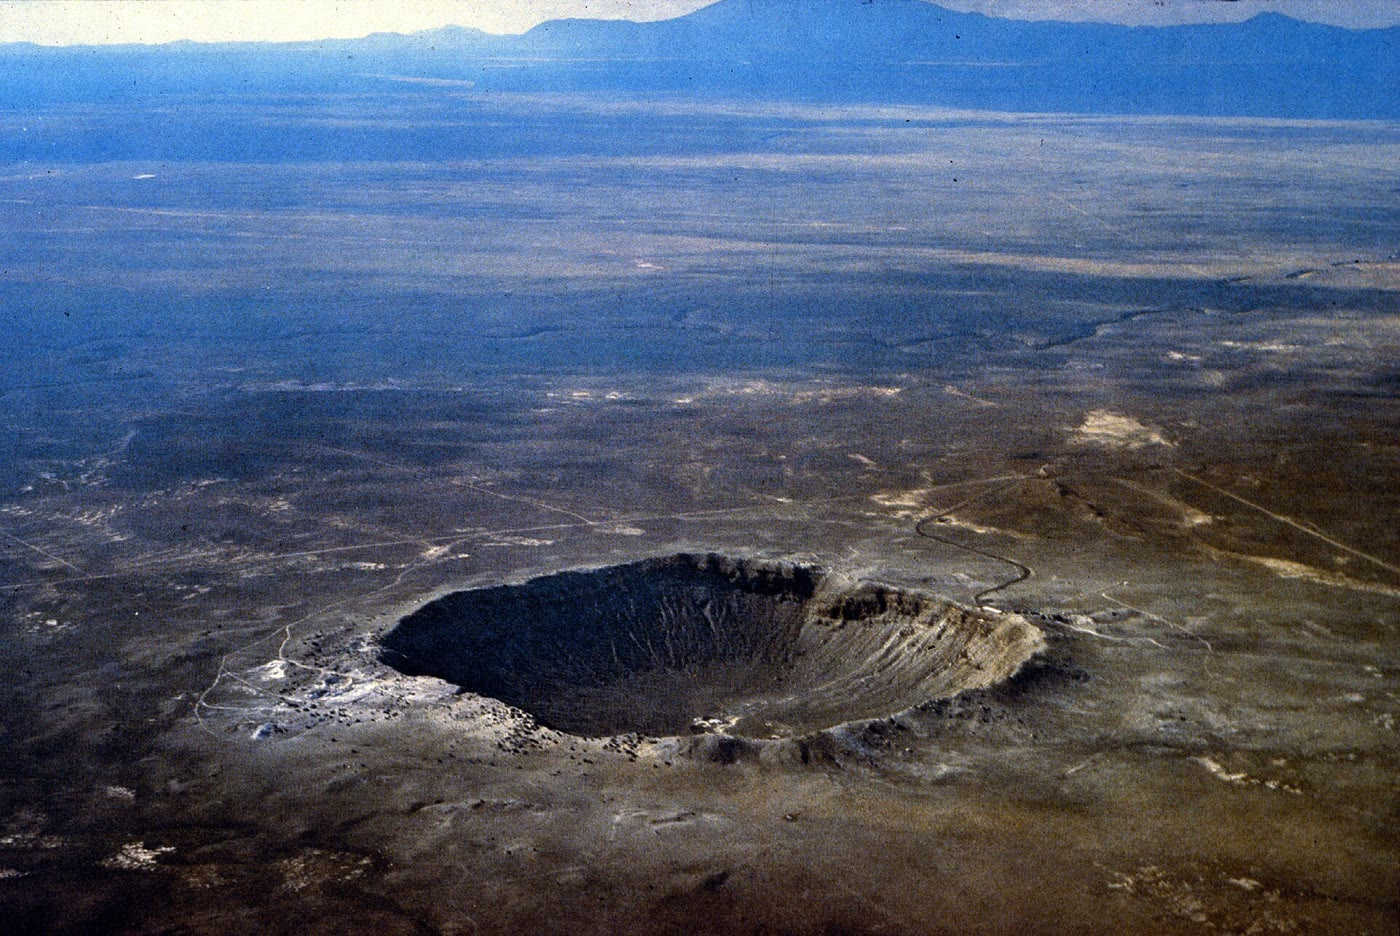
\includegraphics[width=0.66\linewidth]{images/book5/b3-barringer-crater.jpg}
\par\smallskip{\small बैरिंजर मीटियर क्रेटर, एरिज़ोना, एक \omterm{def:b3:planetary-interiors-surfaces:crater-morphology}{सरल क्रेटर}
\qty{1.2}{km} चौड़ा, लगभग 50,000 वर्ष पहले एक लौह उल्कापिंड से बना
लगभग \qty{30}{m} चौड़े; किनारा पठार से ऊपर उठा है और \omterm{def:b3:planetary-interiors-surfaces:crater-morphology}{इजेक्टा-आवरण}
उसके चारों ओर फैला है। हवाई फ़ोटो, USGS/D.~Roddy, सार्वजनिक
डोमेन।}\label{fig:b3:planetary-interiors-surfaces:barringer}
\end{omfigure}
% ledger: photo:b3-barringer, french:barringer

\qty{1}{km} चौड़े क्रेटर का उत्खनन लगभग छह सेकंड में होता है, जबकि
\qty{200}{km} चौड़े का लगभग डेढ़ मिनट में होता है। एक संघट्ट कितने आकार का क्रेटर
बनाता है, वह यह प्रक्षेप्य की ऊर्जा, गुरुत्व और
चट्टान की सामर्थ्य पर निर्भर करता है; इन्हें जोड़ने वाले नियम प्रयोगों
और विस्फोटों से मिलाए गए हैं, विमाहीन समूहों के गुणनफलों के रूप में
व्यक्त होते हैं, और उन्हें यहाँ स्वीकार किया जाता है। उनका सार ऊर्जाओं के संतुलन में है।
% ledger: french:transient

\begin{proposition}[गुरुत्व-शासन का मापन]\label{prop:b3:planetary-interiors-surfaces:scaling}
यदि संघट्ट ऊर्जा $E$ का एक नियत भाग उत्खनित चट्टान को, जिसका घनत्व $\rho$ है,
गुरुत्व $g$ के विरुद्ध ऊपर उठाता है, तो क्रेटर का व्यास इस प्रकार बढ़ता है
\[
  D \propto \left(\frac{E}{\rho g}\right)^{1/4} .
\]
\end{proposition}

\begin{proof}
उत्खनित आयतन $D^3$ के अनुपात में बदलता है, उसका द्रव्यमान $\rho D^3$ है, और
उसे $D$ की कोटि की ऊँचाई तक उठाया जाता है: कार्य $\rho g D^4$ की कोटि का है, जो
$E$ के समानुपाती है।
\end{proof}

ऊर्जा का कुछ भाग ऊष्मा, गलन और चट्टान के टूटने में चला जाता है, इसलिए
वास्तविक नियम इस नियम और सरल नियमों के बीच रहते हैं: पृथ्वी के लिए अक्सर उद्धृत एक तालिका में
क्रेटर को अपने पथरीले
प्रक्षेप्य से बीस गुना चौड़ा लिया गया है। गुरुत्व यह भी तय करता है कि क्रेटर कहाँ सरल नहीं रहता।
क्षणिक कटोरे की दीवारें तब ढह जाती हैं जब उनमें रुकी चट्टान का भार,
जो $\rho g D/3$ की कोटि का है, चट्टान के सामर्थ्य से अधिक हो जाता है, इसलिए
संक्रमण व्यास $1/g$ के अनुसार बदलता है: पृथ्वी पर लगभग \qty{4}{km} क्रिस्टलीय
चट्टान में और \qty{2}{km} अवसादों में, और चंद्रमा पर लगभग \qty{20}{km}, जहाँ
गुरुत्व छह गुना दुर्बल है।
% ledger: french:table21, french:transition, planet:Earth.gravity, planet:Moon.gravity

\section{क्रेटर काल-निर्धारण}\label{sec:b3:planetary-interiors-surfaces:dating}

एकांत छोड़ी गई सतह पर क्रेटर उसी दर से जमा होते हैं जिस दर से पिंड
उससे टकराते हैं। उन्हें गिनने से सतह की आयु ज्ञात होती है, बशर्ते दर ज्ञात हो और
क्रेटर उसी सतह के हों, न कि उसके नीचे की किसी चीज़ के या
किसी पड़ोसी से फेंके गए मलबे के।

\begin{definition}[क्रेटर आकार--आवृत्ति बंटन]\label{def:b3:planetary-interiors-surfaces:sfd}
किसी सतह का \emph{क्रेटर आकार--आवृत्ति बंटन}\index{क्रेटर आकार--आवृत्ति बंटन}
उसके क्रेटरों की वह संख्या $N(D)$ है, जिनका व्यास कम से कम $D$ है, प्रति
इकाई क्षेत्रफल, $D$ के फलन के रूप में (संचयी बंटन), या
व्यास के वर्गों में गिनी गई संख्याएँ, जो सामान्यतः प्रत्येक
पिछले से $\sqrt2$ गुना चौड़ा होता है (वृद्धिशील बंटन)।
\end{definition}

\begin{definition}[क्रेटर काल-निर्धारण; उत्पादन और कालक्रम फलन; साम्य घनत्व]\label{def:b3:planetary-interiors-surfaces:crater-dating}
\emph{क्रेटर काल-निर्धारण}\index{क्रेटर काल-निर्धारण} किसी सतह की आयु को
उसके क्रेटरों के घनत्व से निर्धारित करना है। \emph{क्रेटर उत्पादन
फलन}\index{क्रेटर उत्पादन फलन} वह आकार है जो किसी सतह पर अर्जित क्रेटरों के
आकार--आवृत्ति बंटन का होता है, $F(D) =
N(D)/N(\qty{1}{km})$, जिसे हर आयु पर समान माना जाता है। \emph{क्रेटर
कालक्रम फलन}\index{क्रेटर कालक्रम फलन} $N_1(T)$ वह
\qty{1}{km} और उससे बड़े, प्रति इकाई क्षेत्रफल में जमा हुए क्रेटरों की संख्या है, जो
समय $T$ में जमा होती है। किसी सतह पर किसी दिए गए आकार के क्रेटरों के लिए वह \emph{क्रेटर साम्य
घनत्व}\index{क्रेटर साम्य घनत्व} पर होती है, जब
हर नया क्रेटर औसतन उतने ही पुराने क्रेटर मिटा देता है जितने वह जोड़ता है:
उनकी संख्या और नहीं बढ़ती।
\end{definition}

किसी सतह की मॉडल आयु एक ही गिनती से निकलती है: किसी भी आकार पर मापा गया $N(D)$
$D$ पर यह $N_1 = N(D)/F(D)$ देता है, और $T$ का वह मान ज्ञात होता है जो $N_1(T) = N_1$ को हल करता है। ये
$N(D) = N_1(T)F(D)$ रेखाएँ, स्थिर $T$ के लिए, समकालरेखाएँ कहलाती हैं। मंगल के लिए, व्यापक रूप से प्रयुक्त एक
उत्पादन फलन $\log_{10}D$ में घात~11 का बहुपद है, और
कालक्रम फलन का रूप यह है
\[
  N_1(T) = a\left(e^{bT} - 1\right) + cT , \qquad
  a = \qty{3.22e-14}{km^{-2}}, \ b = \qty{6.93}{Ga^{-1}}, \
  c = \qty{4.875e-4}{km^{-2}.Ga^{-1}} ,
\]
अंतिम तीन अरब वर्षों में यह रैखिक है, उससे पहले तीव्र चरघातांकी।
चंद्रमा का फलन उसी रूप का है, जिसमें $a = \num{5.44e-14}$ और $c =
\num{8.38e-4}$ हैं। यह अपोलो और लूना अवतरण
स्थलों की आयुओं पर फिट किया गया था; मंगल का फलन चंद्रमा का है, जिसे
मंगल और चंद्रमा पर क्रेटर-निर्माण दरों के अनुपात के एक अनुमान से मापा गया है।
% ledger: craterstats:mars-pf, craterstats:mars-cf, craterstats:moon-cf, marchi:neukum

\begin{omfigure}
\centering
\begin{tikzpicture}
\begin{groupplot}[group style={group size=2 by 1, horizontal sep=1.6cm},
  width=0.48\linewidth, height=0.46\linewidth,
  tick label style={font=\scriptsize}, label style={font=\small}, title style={font=\small}]
\nextgroupplot[title={मंगल पर समकालरेखाएँ}, xmode=log, ymode=log, xmin=0.1, xmax=100,
  ymin=1e-8, ymax=100, xlabel={क्रेटर व्यास $D$ (\unit{km})},
  ylabel={$N(D)$, क्रेटर $\geq D$ प्रति \unit{km^2}},
  xtick={0.1,1,10,100}, xticklabels={0.1,1,10,100},
  ytick={1e-8,1e-6,1e-4,1e-2,1}]
\addplot[thick, black!50, dashed] table[x=D, y=eq] {figdata/out/bachelor-3-crater_sfd-iso.dat};
\addplot[omDef] table[x=D, y=N_0.1] {figdata/out/bachelor-3-crater_sfd-iso.dat};
\addplot[omDef] table[x=D, y=N_1] {figdata/out/bachelor-3-crater_sfd-iso.dat};
\addplot[omDef] table[x=D, y=N_3.5] {figdata/out/bachelor-3-crater_sfd-iso.dat};
\addplot[red!70!black, thick] table[x=D, y=N_4] {figdata/out/bachelor-3-crater_sfd-iso.dat};
\node[font=\tiny, omDef, anchor=north east] at (axis cs:0.75,8e-6) {0.1~Ga};
\node[font=\tiny, omDef, anchor=north east] at (axis cs:2.6,1e-5) {1~Ga};
\node[font=\tiny, omDef, anchor=north east] at (axis cs:9,3.5e-5) {3.5~Ga};
\node[font=\tiny, red!70!black, anchor=north east] at (axis cs:45,2.5e-5) {4~Ga};
\node[font=\tiny, black!60, anchor=south, rotate=-30] at (axis cs:25,3.5e-4) {साम्य};
\nextgroupplot[title={कालक्रम फलन}, ymode=log, xmin=0, xmax=4.5,
  ymin=1e-5, ymax=0.3, xlabel={आयु $T$ (\unit{Ga})}, ylabel={$N_1$ प्रति \unit{km^2}},
  legend style={font=\scriptsize, at={(0.03,0.97)}, anchor=north west}]
\addplot[thick, red!70!black] table[x=T, y=mars] {figdata/out/bachelor-3-crater_sfd-chron.dat};
\addlegendentry{मंगल}
\addplot[thick, black!60, dashed] table[x=T, y=moon] {figdata/out/bachelor-3-crater_sfd-chron.dat};
\addlegendentry{चंद्रमा}
\end{groupplot}
\end{tikzpicture}
\par\smallskip{\small बाईं ओर: मंगल की समकालरेखाएँ, यानी संचयी क्रेटर-घनत्व
0.1, 1, 3.5 और 4 अरब वर्ष पुरानी सतहों पर क्रेटरों के, साथ में
साम्य घनत्व (बिंदीदार), जो हर गणना को सीमित करता है: 4
अरब वर्ष पुरानी सतह पर \qty{0.7}{km} से छोटे क्रेटर साम्य पर हैं
और अब आयु का अभिलेख नहीं रखते। दाईं ओर: मंगल और चंद्रमा के कालक्रम फलन,
यानी \qty{1}{km} और उससे बड़े क्रेटरों की संख्या प्रति
वर्ग किलोमीटर, सतह की आयु के
विरुद्ध।}\label{fig:b3:planetary-interiors-surfaces:sfd}
\end{omfigure}
% ledger: craterstats:mars-pf, craterstats:mars-cf, craterstats:moon-cf, craterstats:equilibrium

क्रेटर यादृच्छिक रूप से और एक-दूसरे से स्वतंत्र रूप से बनते हैं, इसलिए
किसी क्षेत्र पर मिली संख्या $n$ एक पॉइसन चर है।

\begin{proposition}[मॉडल आयु की गणना-त्रुटि]\label{prop:b3:planetary-interiors-surfaces:poisson}
यदि $n$ क्रेटर किसी क्षेत्र $A$ पर गिने जाते हैं, तो घनत्व $N = n/A$ का
मानक विचलन $\sqrt n/A$, सापेक्ष त्रुटि $1/\sqrt n$, और मॉडल
आयु का मानक विचलन
\[
  \sigma_T = \frac{N_1(T)}{\sqrt n\,N_1'(T)} .
\]
\end{proposition}

\begin{proof}
पॉइसन चर, जिसका माध्य $\lambda$ है, उसका प्रसरण $\lambda$ होता है, जिसका अनुमान
$n$ से लगाया जाता है। आयु $T = N_1^{-1}(N_1)$ है; प्रथम कोटि तक $\sigma_T =
\sigma_{N_1}/N_1'(T)$ है, और $\sigma_{N_1} = N_1/\sqrt n$ है।
\end{proof}

केवल गिनती की सापेक्ष त्रुटि सौ क्रेटरों के लिए
दस प्रतिशत है। किसी तरुण सतह पर, जहाँ $N_1$ रैखिक है, आयु यही त्रुटि ग्रहण करती है:
$\sigma_T/T = 1/\sqrt n$। किसी पुरानी सतह पर तीव्र फलन इसे
\qty{3.8}{Ga} पर छह गुना घटा देता है (\cref{exo:b3:planetary-interiors-surfaces:11} देखिए);
पुरानी सतहों की मॉडल आयु तब इसके बजाय
फलन के अंशांकन से ही सीमित होती है। गिनती पर दो और सीमाएँ लागू होती हैं। छोटे क्रेटर
संतृप्त हो जाते हैं: सबसे पुरानी सतहों पर लगभग \qty{0.7}{km} से छोटे \omterm{def:b3:planetary-interiors-surfaces:crater-dating}{क्रेटर साम्य घनत्व} पर पहुँच जाते हैं और
समय अंकित करना बंद कर देते हैं। और कोई सतह मिटे बिना नवीकृत हो सकती है:
एक लावा प्रवाह, जो छोटे क्रेटरों को दबा दे, पर बड़े क्रेटरों के किनारों को नहीं,
एक ऐसा बंटन छोड़ जाता है जिसमें मोड़ है: बड़े $D$ पर पुराना और छोटे $D$ पर
तरुण। यह मोड़ \omterm{def:b3:planetary-interiors-surfaces:resurfacing}{पुनःसतहीकरण} की तिथि बताता है।
% ledger: craterstats:equilibrium

\begin{definition}[पुनःसतहीकरण]\label{def:b3:planetary-interiors-surfaces:resurfacing}
\emph{पुनःसतहीकरण}\index{पुनःसतहीकरण} किसी ग्रहीय सतह का नवीकरण है,
लावा, अवसाद, हिम या विरूपण से होने वाला, जो उसके क्रेटरों को हटा देता है या दबा देता है और
उसकी क्रेटर-घड़ी को पुनः शून्य कर देता है।
\end{definition}

\section{पृथ्वी से परे ज्वालामुखीयता और विवर्तनिकी}\label{sec:b3:planetary-interiors-surfaces:volcanism}

हर स्थलीय ग्रह अपनी आंतरिक ऊष्मा अपने स्थलमंडल के माध्यम से खोता है।
पृथ्वी यह गतिमान प्लेटों से करती है; अन्य ग्रह इसे भिन्न तरीके से करते हैं।

\begin{definition}[स्थिर ढक्कन]\label{def:b3:planetary-interiors-surfaces:stagnant-lid}
कोई ग्रह \emph{स्थिर ढक्कन}\index{स्थिर ढक्कन} वाला होता है जब उसका स्थलमंडल
एक ही कठोर कवच हो जो नीचे के प्रावार के संवहन में भाग नहीं लेता:
ऊष्मा उसे चालन से और उसमें से ऊपर उठने वाले मैग्मा से पार करती है।
पृथ्वी जैसे गतिशील-ढक्कन वाले ग्रह पर स्थलमंडल
टूटकर उन प्लेटों में बंट जाता है जो प्रावार में फिर से धंस जाती हैं।
\end{definition}

\begin{definition}[ऊष्मा-नलिका ज्वालामुखीयता]\label{def:b3:planetary-interiors-surfaces:heat-pipe}
\emph{ऊष्मा-नलिका ज्वालामुखीयता}\index{ऊष्मा-नलिका ज्वालामुखीयता} किसी ग्रह की आंतरिक ऊष्मा का
मुख्यतः उस तरीके से खोना है जिसमें मैग्मा संकरी नलिकाओं से ऊपर उठकर
सतह पर उद्गार करता है, जहाँ लावा ठंडा होकर बाद के लावा से दब जाता है:
स्थलमंडल ऊपर से बनता है और ठंडा होकर नीचे ले जाया जाता है।
\end{definition}

\begin{omfigure}
\centering
\begin{tikzpicture}[x=0.5cm, y=0.5cm, font=\scriptsize, >=stealth]
\foreach \dx/\name in {0/गतिशील ढक्कन, 9.5/स्थिर ढक्कन, 19/ऊष्मा नलिका} {
  \begin{scope}[xshift=\dx*0.5cm]
  \fill[orange!15] (0,0) rectangle (8,4);
  \node[anchor=south] at (4,5.6) {\name};
  \end{scope}}
% mobile lid: plates, ridge, slab
\fill[omDef!35] (0,4) rectangle (3.9,4.8);
\fill[omDef!35] (4.1,4) rectangle (6.2,4.8);
\fill[omDef!35] (6.2,4.8) -- (7.6,1.6) -- (6.9,1.4) -- (5.5,4.0) -- cycle;
\fill[omDef!35] (6.55,4) rectangle (8,4.8);
\draw[->, thick] (3.6,5.1) -- (1.6,5.1); \draw[->, thick] (4.4,5.1) -- (6.0,5.1);
\draw[->, red!70!black] (4,1.0) -- (4,3.6);
\draw[black!60, ->] (2.0,3.4) arc (90:270:1.0 and 1.2);
\node[anchor=north] at (4,-0.2) {प्लेटें धंसती हैं};
% stagnant lid
\begin{scope}[xshift=4.75cm]
\fill[omDef!35] (0,3.2) rectangle (8,4.8);
\draw[black!60, ->] (2.4,3.0) arc (90:270:1.2 and 1.2);
\draw[black!60, ->] (5.6,0.6) arc (-90:90:1.2 and 1.2);
\fill[red!70!black] (3.9,3.2) rectangle (4.1,4.8);
\fill[red!70!black] (3.0,4.8) -- (4,5.4) -- (5.0,4.8) -- cycle;
\node[anchor=north] at (4,-0.2) {एक मोटा कवच};
\end{scope}
% heat pipe
\begin{scope}[xshift=9.5cm]
\fill[omDef!35] (0,1.0) rectangle (8,4.8);
\foreach \x in {1.5,4,6.5} {\fill[red!70!black] (\x-0.1,1.0) rectangle (\x+0.1,4.8);
  \fill[red!70!black] (\x-0.6,4.8) -- (\x,5.2) -- (\x+0.6,4.8) -- cycle;}
\draw[->, thick] (2.75,4.3) -- (2.75,1.6); \draw[->, thick] (5.25,4.3) -- (5.25,1.6);
\node[anchor=north] at (4,-0.2) {लावा दबा, ढक्कन ठंडा};
\end{scope}
\end{tikzpicture}
\par\smallskip{\small ऊष्मा खोने के तीन तरीके (योजनाबद्ध)। बाएँ: गतिशील
ढक्कन, जिसमें कटकों पर प्लेटें बनती हैं और खाइयों पर धंसती हैं, जैसा पृथ्वी पर होता है।
बीच में: \omterm{def:b3:planetary-interiors-surfaces:stagnant-lid}{स्थिर ढक्कन}, संवहनी प्रावार के ऊपर एक कठोर कवच,
जिसे कुछ दीर्घजीवी ज्वालामुखियों का मैग्मा पार करता है। दाएँ: ऊष्मा-नलिकाएँ,
जिनमें मैग्मा मोटे ठंडे स्थलमंडल से होकर संकरी नलिकाओं में ऊपर उठता है, उसका लावा
बाद के लावा से दबकर
नीचे ले जाया जाता है।}\label{fig:b3:planetary-interiors-surfaces:lids}
\end{omfigure}

मंगल का \omterm{def:b3:planetary-interiors-surfaces:stagnant-lid}{स्थिर ढक्कन} है। प्लेटें न होने के कारण, जो उनके स्रोतों से उन्हें दूर ले जातीं,
उसके ज्वालामुखी टार्सिस उभार पर लंबे समय तक अपनी जगह पर ही बढ़ते रहे।
ओलंपस मॉन्स, सौर तंत्र का ज्ञात सबसे बड़ा ज्वालामुखी, खड़ा है
\qty{27}{km} ऊँचा, जिसका आधार \qty{600}{km} से अधिक चौड़ा है, और उसके चारों ओर
\qty{6}{km} तक ऊँची कगार है; पास के तीन टार्सिस मॉन्टेस में से हर एक 350
से \qty{400}{km} चौड़ा है। इतना बड़ा भार स्थलमंडल को मोड़ देता है, और उसके द्वारा खोदी गई
खाई की चौड़ाई, जैसे पृथ्वी पर, ढक्कन की प्रत्यास्थ मोटाई
बताती है।
% ledger: nasa:olympus-mons

\begin{omfigure}
\centering
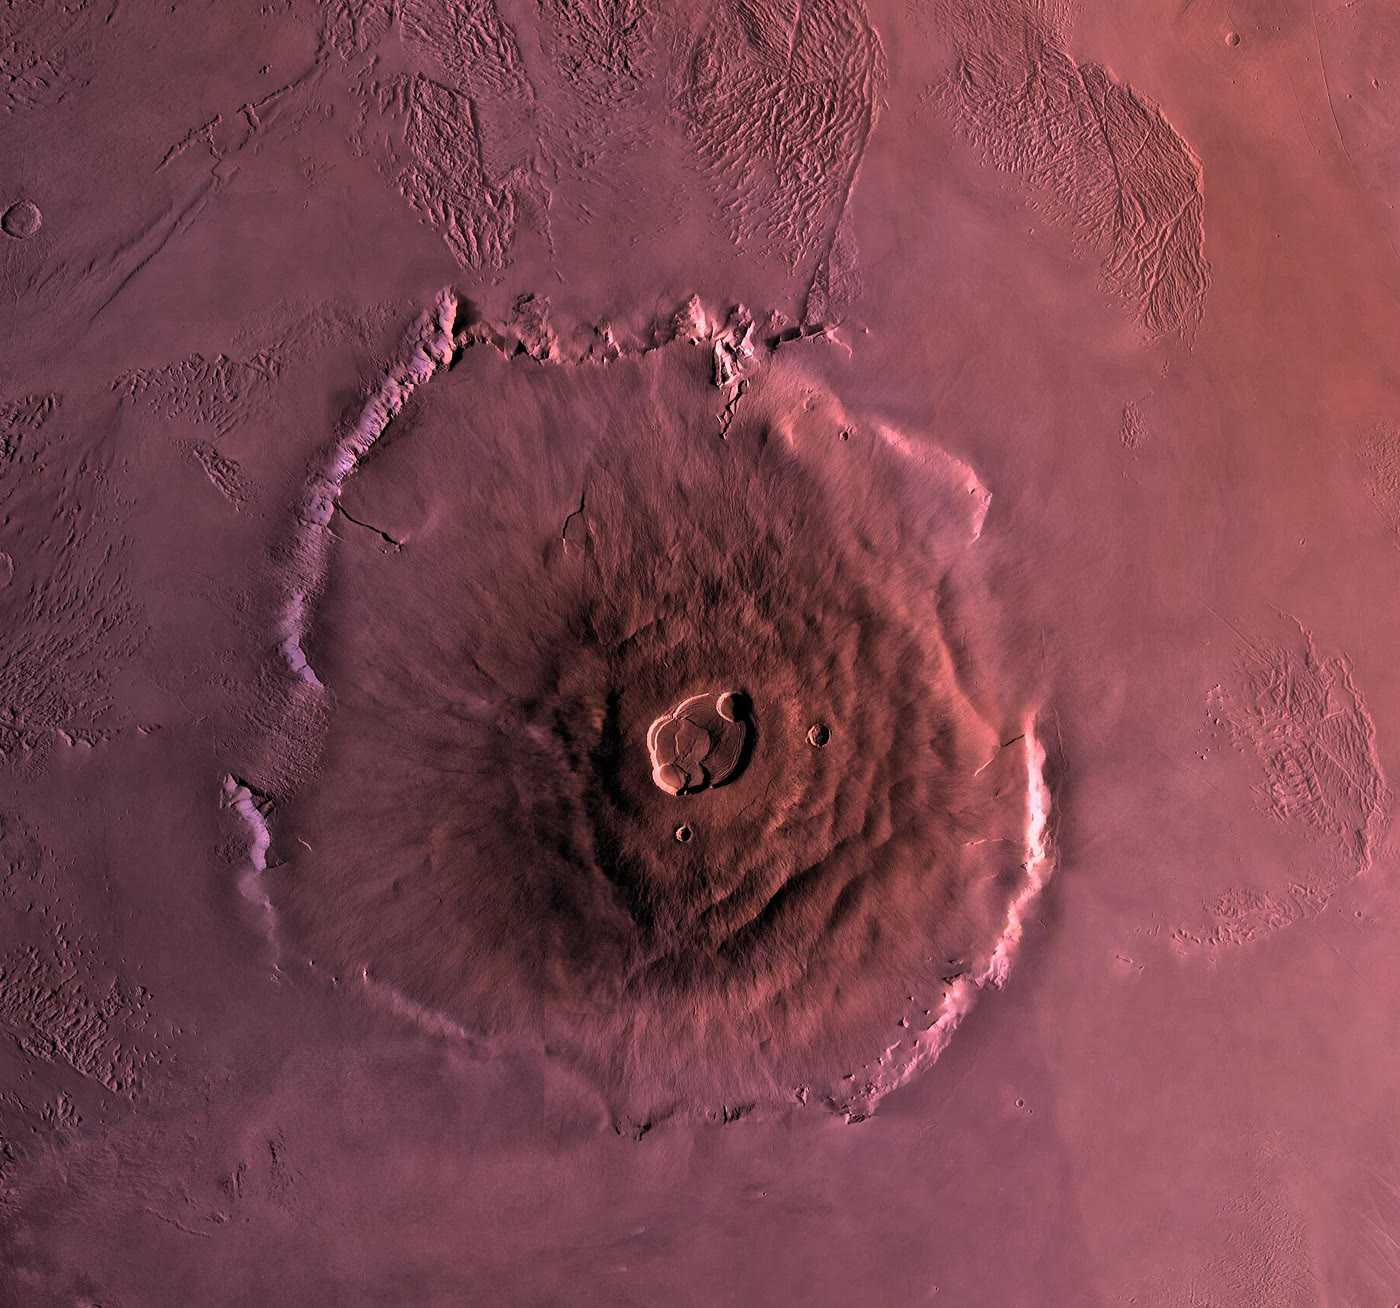
\includegraphics[width=0.48\linewidth]{images/book5/b3-olympus-mons.jpg}
\par\smallskip{\small मंगल पर ओलंपस मॉन्स, वाइकिंग ऑर्बिटरों की छवियों का एक मोज़ेक:
केंद्र में शिखर कैल्डेरा, लावा प्रवाहों के ढलान,
और आधार को घेरने वाली खड़ी कगार, जिसकी चौड़ाई लगभग \qty{600}{km} है।
NASA/JPL/USGS, सार्वजनिक डोमेन।}\label{fig:b3:planetary-interiors-surfaces:olympus}
\end{omfigure}
% ledger: photo:b3-olympus-mons, nasa:olympus-mons

शुक्र, जो आकार में पृथ्वी का जुड़वाँ है, संघट्ट क्रेटरों की संख्या में
पृथ्वी को छोड़कर किसी भी चट्टानी ग्रह से कहीं कम है। उसकी सतह की विशेषताएँ औसतन
150 मिलियन वर्ष जितनी तरुण हो सकती हैं, उनके बीच कुछ पुराने टुकड़े हैं:
ज्वालामुखीयता और विरूपण ने उसकी अधिकांश सतह को नवीकृत किया, शायद टुकड़ों में
और लंबे समय में, शायद अधिक तेज़ी से। शुक्र पर हज़ारों ज्वालामुखी हैं
और प्लेटों के गतिमान होने का कोई संकेत नहीं।
% ledger: nasa:venus-surface, planet:Venus.diameter, planet:Earth.diameter

आयो, बृहस्पति का सबसे अंदरूनी बड़ा उपग्रह, अपनी सतह से
\qty{2.5}{W.m^{-2}} से अधिक ऊष्मा खोता है, जो पृथ्वी के औसत
\qty{0.092}{W.m^{-2}} से लगभग 27 गुना है। इसकी ऊष्मा रेडियोधर्मिता
की नहीं है: यह ज्वारों द्वारा उत्पन्न होती है।
% ledger: veeder:io-heat, dd10:split

\begin{definition}[ज्वारीय ऊष्मन]\label{def:b3:planetary-interiors-surfaces:tidal-heating}
\emph{ज्वारीय ऊष्मन}\index{ज्वारीय ऊष्मन} वह ऊष्मा है जो किसी पिंड के भीतर
उस विरूपण के घर्षण से उत्पन्न होती है, जो एक बदलता हुआ ज्वार उस पर डालता है।
उत्केंद्र कक्षा में तुल्यकाली घूर्णन करने वाला एक उपग्रह अपने ग्रह के ज्वार को
हर कक्षा के दौरान प्रबलता में बदलता और आगे-पीछे झूलता हुआ देखता है।
\end{definition}

\begin{proposition}[तुल्यकाली उपग्रह की ज्वारीय शक्ति]\label{prop:b3:planetary-interiors-surfaces:tidal-power}
त्रिज्या $R$ वाला एक उपग्रह, जो तुल्यकाली घूर्णन करता है, माध्य गति
$n$ और छोटी उत्केंद्रता $e$ वाली कक्षा में, निम्नलिखित शक्ति का क्षय करता है:
\[
  \dot E = \frac{21}{2}\,\frac{k_2}{Q}\,\frac{(nR)^5}{G}\,e^2 ,
\]
जहाँ $Q$ उपग्रह का ज्वारीय गुण-गुणक है, इसलिए $k_2/Q$
ज्वारीय विरूपण के उस भाग को मापता है जो ऊष्मा के रूप में खो जाता है।
\end{proposition}

यह प्रतिज्ञप्ति स्वीकार की जाती है। ऊर्जा का क्षय करने वाले ज्वार कक्षा को वृत्ताकार भी बना देते हैं;
परंतु आयो की कक्षा दीर्घवृत्तीय ही रहती है, जिसकी उत्केंद्रता 0.004 है, क्योंकि
यूरोपा और गैनीमीड के सटीक समय पर लगने वाले खिंचाव उसे विक्षुब्ध करते हैं, और उनके
कक्षीय आवर्तकाल \num{1.77}, \num{3.55} और \num{7.15}~दिन लगभग ठीक
1:2:4 के अनुपात में रहते हैं (\cref{exo:b3:planetary-interiors-surfaces:8} देखिए)। इसकी सतह
हर कक्षा में \qty{100}{m} तक ऊपर-नीचे होती है। ज्वालामुखी
आयो को लावा से इतनी तेज़ी से ढकते हैं कि उस पर क्रेटर बन नहीं पाते;
इसकी ऊष्मा कैसे निकलती है, इसका एक मॉडल \omterm{def:b3:planetary-interiors-surfaces:heat-pipe}{ऊष्मा-नलिका ज्वालामुखीयता} है, जो एक मोटा,
ठंडा स्थलमंडल इसकी दहकती सतह के नीचे बनाए रखेगा।
% ledger: nasa:galilean-orbits, beuthe:tidal-power, nasa:io-orbit, nasa:io-facts

\begin{definition}[उपसतही महासागर]\label{def:b3:planetary-interiors-surfaces:ocean-world}
\emph{उपसतही महासागर}\index{उपसतही महासागर} किसी उपग्रह या बौने ग्रह की बर्फ़ की परत के नीचे
द्रव जल की एक वैश्विक परत है, जो ज्वारीय और
रेडियोजेनिक ऊष्मा से द्रव अवस्था में बनी रहती है।
\end{definition}

\begin{definition}[हिम-ज्वालामुखीयता]\label{def:b3:planetary-interiors-surfaces:cryovolcanism}
\emph{हिम-ज्वालामुखीयता}\index{हिम-ज्वालामुखीयता} जल, लवणीय घोल
या अन्य वाष्पशील द्रवों और वाष्पों का, पिघली चट्टान के बजाय,
किसी उपग्रह या बौने ग्रह की बर्फ़ीली सतह पर उद्गार है।
\end{definition}

यूरोपा की बर्फ़ की परत, जिसे जूनो यान के माइक्रोवेव रेडियोमीटर ने
उस क्षेत्र में मापा जिसके ऊपर से वह उड़ा, औसतन लगभग \qty{29}{km} मोटी है;
उसके नीचे एक खारा महासागर है, जिसमें पृथ्वी के सभी
महासागरों के कुल जल से दोगुना जल है। शनि के उपग्रह एन्सेलेडस पर, जो केवल लगभग \qty{500}{km}
चौड़ा है, कैसिनी यान ने 2005 में बर्फ़ के कणों और गैस के फ़व्वारे पाए,
जो दक्षिणी ध्रुव के पास गर्म भ्रंशों से निकलते हैं, लगभग
\qty{400}{m.s^{-1}} की गति से। इसके गुरुत्व और इसके घूर्णन की डगमगाहट से पता चला
कि ये फ़व्वारे एक वैश्विक महासागर से जल लेते हैं, जो औसतन 20 से
\qty{25}{km} मोटी बर्फ़ की परत के नीचे है और दक्षिणी ध्रुव पर संभवतः केवल 1 से
\qty{5}{km} मोटी है।
% ledger: jpl:europa-shell, nasa:europa-ocean, nasa:enceladus

\section{बड़े क्रोड और छोटे क्रोड}\label{sec:b3:planetary-interiors-surfaces:cores}

मापे गए चार क्रोड एक अजीब परिवार बनाते हैं। अपनी त्रिज्या के सापेक्ष, पृथ्वी का
क्रोड सतह की ओर 0.55 दूरी तक पहुँचता है और मंगल का 0.54;
चंद्रमा का 0.19; बुध का 0.82। पुस्तक 4 (स्नातक वर्ष 2) में बताया गया विभेदन
प्रत्येक पिंड के भीतर धातु को सिलिकेट से अलग करता है, पर धातु के अनुपात को
इतना भिन्न नहीं बना सकता। यह काम विशाल संघट्ट कर सकते हैं। माना जाता है कि चंद्रमा
लगभग 4.5 अरब वर्ष पहले मंगल के आकार के एक पिंड और युवा पृथ्वी की टक्कर के मलबे से बना;
संघट्टक की धातु पृथ्वी के क्रोड में मिल गई, जबकि चंद्रमा ने अधिकतर प्रावार की चट्टान बटोरी,
इसीलिए उसका क्रोड छोटा है। इसी प्रकार के संघट्टों ने बुध के सिलिकेट प्रावार का
बड़ा भाग छीन लिया होगा और उसे लौह-समृद्ध ग्रह बना दिया होगा, जिसका क्रोड
उसके अधिकांश भाग को भरता है। क्रोड, क्रेटरों की तरह, टक्करों का
इतिहास दर्ज करते हैं।
% ledger: data:prem, jpl:insight-interior, nasa:moon-core, agu:mercury-core, french:giant-impacts

\section{अभ्यास}

\begin{exercise}[$\star$]\label{exo:b3:planetary-interiors-surfaces:1}
बुध का माध्य घनत्व \qty{5429}{kg.m^{-3}} है, जड़त्व-आघूर्ण
गुणक 0.35 और त्रिज्या \qty{2440}{km} है। दो-परत मॉडल से, जिसमें प्रावार का
घनत्व \qty{3300}{kg.m^{-3}} है, क्रोड की सापेक्ष त्रिज्या
उसकी त्रिज्या किलोमीटर में और उसका घनत्व परिकलित कीजिए।
\end{exercise}

\begin{exercise}[$\star$]\label{exo:b3:planetary-interiors-surfaces:2}
\qty{50}{m} व्यास का एक पथरीला प्रक्षेप्य, जिसका घनत्व \qty{3500}{kg.m^{-3}} है,
\qty{20}{km.s^{-1}} की गति से पृथ्वी से ऊर्ध्वाधर टकराता है। इसका द्रव्यमान और
उसकी गतिज ऊर्जा ज्यूल में और विस्फोटक के मेगाटन में
($\qty{1}{Mt} = \qty{4.2e15}{J}$) परिकलित कीजिए। बीस प्रक्षेप्य-व्यास के नियम से
कितने व्यास का क्रेटर प्राप्त होता है?
\end{exercise}

\begin{exercise}[$\star$]\label{exo:b3:planetary-interiors-surfaces:3}
मंगल के एक मैदान पर, जिसका क्षेत्रफल \qty{100000}{km^2} है, 120 क्रेटर \qty{1}{km} और
उससे बड़े गिने जाते हैं। $N_1$, उसकी सापेक्ष त्रुटि और मैदान की मॉडल आयु
उसकी त्रुटि के साथ परिकलित कीजिए।
\end{exercise}

\begin{exercise}[$\star$]\label{exo:b3:planetary-interiors-surfaces:4}
आयो, जिसकी त्रिज्या \qty{1821.5}{km} है, \qty{2.5}{W.m^{-2}} की दर से ऊष्मा खोता है। उसकी
कुल ऊष्मा हानि परिकलित कीजिए और पृथ्वी की \qty{47}{TW} से उसकी तुलना कीजिए,
कुल में और प्रति वर्ग मीटर (\qty{0.092}{W.m^{-2}}) में।
\end{exercise}

\begin{exercise}[$\star\star$]\label{exo:b3:planetary-interiors-surfaces:5}
मंगल का द्रव्यमान \qty{6.417e23}{kg} और त्रिज्या \qty{3389.5}{km} है।
(क)~उसका माध्य घनत्व, पृष्ठीय गुरुत्व और $\rho gR$ परिकलित कीजिए।
(ख)~उसे एकसमान असंपीड्य गोला मानते हुए, जिसकी दृढ़ता
\qty{67}{GPa} है, उसकी \omterm{def:b3:planetary-interiors-surfaces:love-number}{लव संख्या} $k_2$ परिकलित कीजिए। (ग)~मापा गया मान
$0.153 \pm 0.017$ है। तुलना क्या दर्शाती है?
\end{exercise}

\begin{exercise}[$\star\star$]\label{exo:b3:planetary-interiors-surfaces:6}
पृथ्वी पर ($g = \qty{9.8}{m.s^{-2}}$) सरल से \omterm{def:b3:planetary-interiors-surfaces:crater-morphology}{जटिल क्रेटर} का संक्रमण
क्रिस्टलीय चट्टान में लगभग \qty{4}{km} पर और
अवसाद में \qty{2}{km} पर होता है। (क)~मान लीजिए कि संक्रमण-व्यास $1/g$ के अनुपात में बदलता है,
चंद्रमा पर ($g = \qty{1.62}{m.s^{-2}}$) और मंगल तथा
बुध पर ($g = \qty{3.7}{m.s^{-2}}$) पूर्वानुमान लगाइए; उसकी तुलना
चंद्रमा पर देखे गए \qty{20}{km} से कीजिए। (ख)~यदि ढहना तब शुरू होता है जब $\rho gD/3$
चट्टान की सामर्थ्य $Y$ से अधिक हो, तो पृथ्वी का क्रिस्टलीय संक्रमण
किस सामर्थ्य का मान देता है, $\rho = \qty{2600}{kg.m^{-3}}$ के लिए?
\end{exercise}

\begin{exercise}[$\star\star$]\label{exo:b3:planetary-interiors-surfaces:7}
एक पृष्ठ पर \qty{1}{km} और उससे अधिक व्यास के $\num{2.0e-3}$ क्रेटर
प्रति वर्ग किलोमीटर हैं। मंगल का \omterm{def:b3:planetary-interiors-surfaces:crater-dating}{क्रेटर कालक्रम फलन} से इसकी मॉडल आयु
समीकरण को संख्यात्मक रूप से हल करके ज्ञात कीजिए। चंद्र फलन से कौन-सी आयु प्राप्त होती,
और दोनों को आपस में क्यों नहीं बदला जा सकता?
\end{exercise}

\begin{exercise}[$\star\star$]\label{exo:b3:planetary-interiors-surfaces:8}
आयो, यूरोपा और गैनिमीड के कक्षीय आवर्तकाल 1.769138, 3.551181 और
\num{7.154553}~दिन हैं। (क)~क्रमागत आवर्तकालों के अनुपात परिकलित कीजिए।
(ख)~$1/P_I - 3/P_E + 2/P_G$ परिकलित कीजिए और टिप्पणी कीजिए। (ग)~अनुनाद
क्यों वह उत्केंद्रता बनाए रख सकता है जिसे अन्यथा ज्वार हटा देते हैं?
\end{exercise}

\begin{exercise}[$\star\star$]\label{exo:b3:planetary-interiors-surfaces:9}
आयो \num{1.769138}~दिन में बृहस्पति की परिक्रमा करता है, जिसकी उत्केंद्रता 0.004 है।
$k_2/Q$ की प्रति इकाई पर ज्वारीय-शक्ति प्रस्ताव से मिलने वाली शक्ति परिकलित कीजिए,
और वह $k_2/Q$ मान ज्ञात कीजिए जिससे आयो की ऊष्मा-हानि की आपूर्ति हो सके,
जो \cref{exo:b3:planetary-interiors-surfaces:4} में है।
\end{exercise}

\begin{exercise}[$\star\star\star$]\label{exo:b3:planetary-interiors-surfaces:10}
चंद्रमा के लिए $\bar\rho = \qty{3340}{kg.m^{-3}}$ और $C = 0.394$।
(क)~दर्शाइए कि द्वि-परत मॉडल में $\mathrm dx^2/\mathrm dC =
\tfrac52\bar\rho/(\bar\rho - \rho_m)$ स्थिर $\rho_m$ पर सत्य है। (ख)~वह प्रावार घनत्व
जो $x = 0.19$ का क्रोड देता है, \qty{3288}{kg.m^{-3}}, लेकर
$x$ और $\rho_c$ क्या हैं, जब $C = 0.395$ और जब $C = 0.393$?
(ग)~जड़त्व आघूर्ण से एक छोटे क्रोड को आँकने के बारे में यह
क्या कहता है?
\end{exercise}

\begin{exercise}[$\star\star\star$]\label{exo:b3:planetary-interiors-surfaces:11}
(क)~100 क्रेटरों के लिए, \qty{1.0}{Ga} पुराने मंगल-पृष्ठ और
\qty{3.8}{Ga} पुराने एक पृष्ठ की मॉडल आयु की गणना-त्रुटि परिकलित कीजिए।
(ख)~कालक्रम फलन के रैखिक भाग पर दर्शाइए कि $\sigma_T/T =
1/\sqrt n$ होता है। (ग)~तब पुराने पृष्ठों की आयुएँ अब भी अनिश्चित क्यों हैं?
\end{exercise}

\begin{exercise}[$\star\star\star$]\label{exo:b3:planetary-interiors-surfaces:12}
त्रिज्या \qty{1560.8}{km} वाला यूरोपा \num{3.551181}~दिन में परिक्रमा करता है,
जिसकी उत्केंद्रता 0.009 है। (क)~यदि यूरोपा ने आयो जैसे $k_2/Q$ के साथ ज्वार का क्षय किया होता,
तो आयो की ज्वारीय शक्ति का कितना भाग वह उत्पन्न करता, और ऊष्मा-प्रवाह कितना होता?
(ख)~बर्फ़ के नीचे महासागर वाले उपग्रह के लिए यह धारणा संदिग्ध क्यों है?
\end{exercise}

\section{समस्या: मंगल के दो मैदान}

\begin{problem}[{सप्ताहांत समस्या --- मंगल का क्रोड और दो
काल्पनिक लावा मैदानों की आयु}]
\label{pb:b3:planetary-interiors-surfaces:1}
मंगल का द्रव्यमान \qty{6.4169e23}{kg}, त्रिज्या \qty{3389.5}{km} और
जड़त्व-आघूर्ण गुणक 0.366 है। दो काल्पनिक मैदान, A और B, इसके
ज्वालामुखीय प्रांतों पर स्थित हैं; उनके क्रेटर
$\sqrt2$ चौड़े खानों में चित्रों पर गिने गए हैं।

\medskip\noindent\textbf{भाग I --- क्रोड।}
\begin{enumerate}
\item मंगल का माध्य घनत्व परिकलित कीजिए।
\item द्वि-परत मॉडल लेकर, जिसमें प्रावार का घनत्व \qty{3500}{kg.m^{-3}} हो,
  क्रोड की सापेक्ष त्रिज्या, उसकी किलोमीटर में त्रिज्या और उसका
  घनत्व परिकलित कीजिए।
\item इनसाइट ने क्रोड की त्रिज्या \qty{1830}{km} मापी। अब द्वि-परत मॉडल
  के लिए प्रावार और क्रोड के कौन-से घनत्व आवश्यक हैं?
\item उस क्रोड-घनत्व की तुलना पृथ्वी के बाह्य क्रोड के घनत्व से कीजिए,
  उसके ठीक ऊपरी शीर्ष पर, जो संदर्भ पृथ्वी मॉडल में \qty{9900}{kg.m^{-3}} है,
  और बताइए कि मंगल के लिए कम मान क्यों अपेक्षित है, और यह और क्या
  संकेत देता है।
\item मंगल की एकसमान-गोला \omterm{def:b3:planetary-interiors-surfaces:love-number}{लव संख्या}, जिसकी दृढ़ता
  \qty{67}{GPa} है, 0.109 होती है; मापा गया मान 0.153 है। कौन-सा प्रेक्षण
  पहले आया, और उसने क्रोड के बारे में पहले ही क्या कहा था?
\item मंगल की भूपर्पटी 20 से \qty{37}{km} मोटी है। ग्रह के आयतन का कितना
  भाग यह धारण करती है? क्या इसे नज़रअंदाज़ करना उचित था?
\end{enumerate}

\medskip\noindent\textbf{भाग II --- मैदान A पर गणनाएँ।} मैदान A का
\qty{80000}{km^2} क्षेत्रफल घेरता है। इसके क्रेटर, व्यास-खानों के अनुसार (km):
\begin{center}
\small
\begin{tabular}{lccccccccc}
\hline
खाना & 1--1.41 & 1.41--2 & 2--2.83 & 2.83--4 & 4--5.66 & 5.66--8 & 8--11.3 & 11.3--16 & 16--22.6 \\
\hline
मैदान A & 38 & 6 & 5 & 3 & 0 & 0 & 0 & 1 & 1 \\
मैदान B & 48 & 8 & 31 & 12 & 7 & 2 & 0 & 2 & 2 \\
\hline
\end{tabular}
\end{center}
\begin{enumerate}[resume]
\item मैदान A की संचयी गणनाएँ, \qty{1}{km} से ऊपर, परिकलित कीजिए।
\item $N(\qty{1}{km})$ प्रति वर्ग किलोमीटर और उसका मानक
  विचलन परिकलित कीजिए।
\item \omterm{def:b3:planetary-interiors-surfaces:crater-dating}{क्रेटर उत्पादन फलन} $F(\qty{2}{km}) = 0.147$ और
  $F(\qty{1.41}{km}) = 0.355$ देता है। क्या \qty{1.41}{km} और \qty{2}{km} पर
  गणनाएँ उत्पादन फलन के आकार से संगत हैं?
\item क्या मैदान A \omterm{def:b3:planetary-interiors-surfaces:crater-dating}{क्रेटर साम्य घनत्व} के निकट कहीं है,
  \qty{1}{km} पर \qty{0.072}{km^{-2}}?
\item खाने $\sqrt2$ चौड़े क्यों चुने गए हैं?
\item छोटे क्रेटरों के गुच्छे और शृंखलाएँ गणना से बाहर रखी जाती हैं। क्यों?
\end{enumerate}

\medskip\noindent\textbf{भाग III --- मॉडल आयु।} मंगल ग्रह के
कालक्रम फलन का उपयोग कीजिए।
\begin{enumerate}[resume]
\item मैदान A की मॉडल आयु परिकलित कीजिए। जाँच कीजिए कि घातांकीय पद
  उपेक्षित किया जा सकता है।
\item इसकी गणना-त्रुटि परिकलित कीजिए।
\item चंद्र कालक्रम से कौन-सी आयु प्राप्त होती?
\item मैदान B का क्षेत्रफल \qty{120000}{km^2} है। इसके \qty{2}{km} और उससे बड़े
  क्रेटरों का उपयोग करके $N(\qty{2}{km})$, फिर $N_1$, और फिर
  समीकरण को संख्यात्मक रूप से हल करके उसकी मॉडल आयु परिकलित कीजिए।
\item उस आयु की गणना-त्रुटि परिकलित कीजिए।
\item दोनों आयुओं की सापेक्ष त्रुटियों की तुलना कीजिए और
  इस अंतर की व्याख्या कीजिए।
\end{enumerate}

\medskip\noindent\textbf{भाग IV --- मैदान B के दबे हुए क्रेटर।}
\begin{enumerate}[resume]
\item यदि मैदान B की पूरी सतह प्रश्न~16 वाली आयु की होती, तो 1 और \qty{2}{km} के बीच के क्रेटर
  उसमें कितने होने चाहिए? उसमें कितने हैं?
\item मान लीजिए कि लावा ने \qty{2}{km} से छोटे प्रत्येक क्रेटर को
  एक समय $T_r$ पर दबा दिया और बड़े क्रेटरों को छोड़ दिया। \num{1}--\qty{2}{km} के
  क्रेटरों से $T_r$ परिकलित कीजिए।
\item $T_r$ की गणना-त्रुटि परिकलित कीजिए।
\item मंगल ग्रह पर एक ताज़ा \omterm{def:b3:planetary-interiors-surfaces:crater-morphology}{सरल क्रेटर} की गहराई उसकी चौड़ाई के
  पाँचवें भाग के बराबर मान लीजिए (यह इस समस्या की एक कल्पना है)। लावा कितना मोटा होना चाहिए कि
  \qty{2}{km} का क्रेटर दब जाए, और बड़े क्रेटर अब भी क्यों दिखते हैं?
\item क्या मैदान B और मैदान A का लावा ज्वालामुखीयता के एक ही
  घटनाक्रम का हिस्सा हो सकता है?
\item मैदान A की मॉडल आयु, अरब वर्षों में और दो सार्थक अंकों तक,
  दीजिए।
\end{enumerate}
\end{problem}
% ledger: nasa:mars, jpl:insight-interior, yoder:mars-k2, data:prem, craterstats:mars-pf, craterstats:mars-cf, craterstats:moon-cf, craterstats:equilibrium
